\documentclass[12pt,ngerman]{dtk}
\usepackage[utf8]{inputenc}
\usepackage{hyperref}
\usepackage{babel}
\usepackage{csquotes}
\usepackage{listings}
\usepackage{xcolor}
\usepackage{microtype}

\usepackage{subfig}

\definecolor{hellgelb}{rgb}{1,1,0.8}
\definecolor{colKeys}{rgb}{0,0,1}
\definecolor{colIdentifier}{rgb}{0,0,0}
\definecolor{colComments}{rgb}{1,0,0}
\definecolor{colString}{rgb}{0,0.5,0}


\lstset{%
    float=hbp,%
    basicstyle=\ttfamily\small, %
    identifierstyle=\color{colIdentifier}, %
    keywordstyle=\color{colKeys}, %
    stringstyle=\color{colString}, %
    commentstyle=\color{colComments}, %
    columns=flexible, %
    tabsize=2, %
%    frame=single, %
    extendedchars=true, %
    showspaces=false, %
    showstringspaces=false, %
    backgroundcolor=\color{hellgelb}, %
    breakautoindent=true, %
    captionpos=b%
}


\title{Die neue \texttt{scrletter} Umgebung in KOMA-Script} 
\Author{Uwe}{Ziegenhagen}{Köln} 
\markboth{\texttt{scrletter} Umgebung}{\texttt{scrletter} Umgebung}


\begin{document}
\maketitle

\begin{abstract}
Seit Version 3.15 von KOMA-Script gibt es die Brief-Funktionalität nicht nur in Form der \texttt{scrlttr2}-Klasse, sondern auch als Paket. Im folgenden Artikel wird kurz beschrieben, wie man dieses \texttt{scrletter}-Paket in eigenen Dokumenten nutzt.
\end{abstract}


\section{Das \texttt{scrletter}-Paket}

Ein Hinweis vorweg: Das Paket hat noch Beta-Status; kleinere, eventuell auch inkompatible Änderungen kann es laut Markus Kohm noch geben. Da ich im täglichen Leben jedoch recht viel mit der \texttt{scrlettr2} Klasse arbeite, wollte ich es unbedingt mal ausprobieren.

Die Nutzung des Pakets ist sehr einfach, ein \verb|\usepackage{scrletter}| in der Präambel des Dokuments reicht aus. Das Dokument selbst muss dabei mit einer der KOMA-Script Klassen (scrartcl, scrreprt oder scrbook) gesetzt werden, eine Nutzung beispielsweise innerhalb von Dokumenten der \enquote{article} Klasse ist nicht vorgesehen. 

Innerhalb des Dokuments kann man dann mit der \texttt{letter}-Umgebung einen neuen Brief einleiten, der verständlicherweise auf eine separate Seite gesetzt wird. Man kann auch die üblichen KOMA-Variablen setzen und im Dokument auswerten lassen. Listing \ref{lis:brief}
zeigt ein entsprechendes Beispiel.

\begin{lstlisting}[language={[LaTeX]TeX},morekeywords={blindtext,setkomavar,opening, closing},basicstyle=\ttfamily\footnotesize,caption={\LaTeX-Datei für die Einbindung der erzeugten Datei},label={lis:brief}]
\documentclass[12pt,ngerman]{scrartcl}
\usepackage[utf8]{inputenc}
\usepackage[T1]{fontenc}
\usepackage{babel}
\usepackage{blindtext}
\usepackage{scrletter}
\begin{document}
\blindtext[3]
\setkomavar{fromname}{Max Mustermann}
\setkomavar{fromaddress}{Musterstr. 12 \\ 12345~Musterstadt}
\setkomavar{place}{Musterstadt}
\setkomavar{subject}{Mahnung}
 
\begin{letter}{Martina Musterfrau \\ Musterweg 4 \\ 12346~Musterdorf}
\opening{Sehr geehrte Damen und Herren,}
 
\closing{Hochachtungsvoll,}
\end{letter}
\end{document}
\end{lstlisting}
 
\begin{figure}[ht]
   \centering
      \subfloat[Seite 1]{\fbox{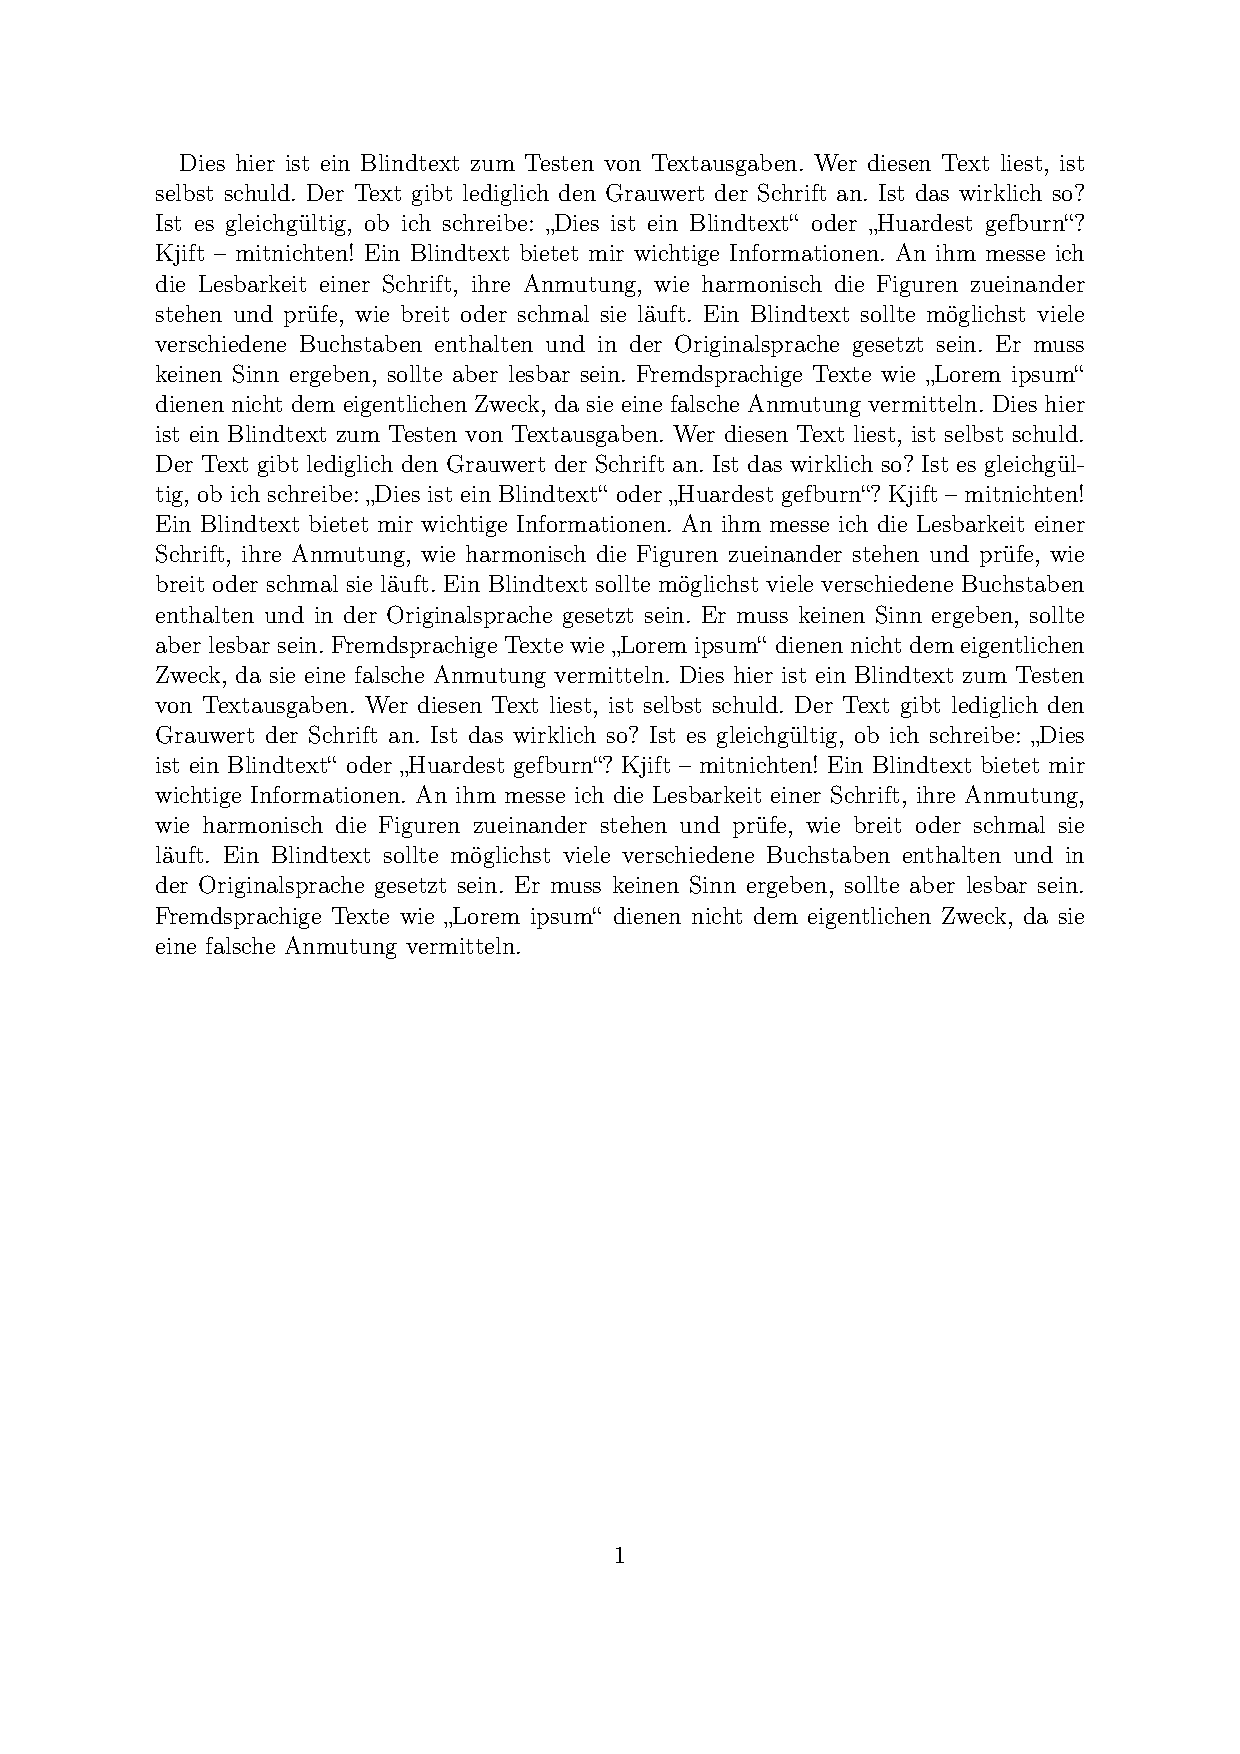
\includegraphics[width=0.45\textwidth,page=1]{scrletter-Beispiel}}}\qquad
      \subfloat[Seite 2]{\fbox{\includegraphics[width=0.45\textwidth,page=2]{scrletter-Beispiel}}}\qquad
   \caption[Ergebnisse]{Die beiden erzeugten Seiten}\label{fig:a}
\end{figure}

Abbildung \ref{fig:a} zeigt die beiden erzeugten Seiten aus dem obigen Listing. Ich selbst habe zwar noch keine konkrete Anwendung für diese Kombination aus Brief und Dokument, denke aber dass es eine Reihe spannender Möglichkeiten bietet.

Ein Hinweis noch aus der Anleitung: Es ist nicht möglich, eine LCO-Datei als Paket-Parameter zu übergeben, für diese Zwecke 
kann man aber die auch in der \texttt{scrlttr2}-Klasse verfügbaren Befehle \verb|\LoadLetterOption| beziehungsweise \verb|\LoadLetterOptions| nutzen. Weitere Unterschiede zwischen Klasse und Paket findet man in Teil II der KOMA-Script-Anleitung.

Alle Nutzer sind übrigens eingeladen, das Paket zu testen, Markus Kohm freut sich über entsprechende Rückmeldungen. Siehe dazu auch die Webseite des Projekts unter \texttt{http://www.komascript.de/scrletter}.

\end{document} 